\documentclass[./main.tex]{subfiles}

\begin{document}

本章我们将解决几个有趣的问题,同时尝试用函数式的方式来解决这些问题。

\subsection*{运算逆波兰表示法}

学校里学习的数学表达式都是中置(infix)表示法,比如 $10 - (4 + 3) * 2$,其中 $+$,$*$,$-$就是中置算子。在 Haskell
中就像是\acode{+}或者\acode{elem}那样。这种写法对于人类来说便于阅读和理解,但是缺点就是必须用括号来描述运算的优先级。

逆波兰法(Reverse Polish notation form)是另一种数学的表示法,上述表达式用 RPN 表达就是 $10\ 4\ 3\ +\ 2\ *\ -$。
可以想象成堆叠,从左往右阅读算式,每当碰到一个数值就把它堆上堆叠。当碰到一个算子,就把两个数值从堆叠上拿下来,运算完成后
再将结果堆上堆叠。

\begin{figure}[h]
  \centering
  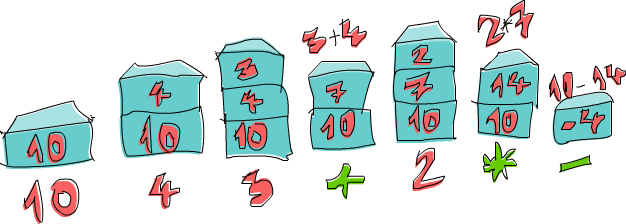
\includegraphics[width=0.9\textwidth]{\subfix{./images/rpn.png}}
\end{figure}

\begin{anote}
  在实现一个函数之前,更重要的是思考其类型声明。在 Haskell 中,一个函数的类型声明能告诉我们很多函数的信息,感谢强壮的
  类型系统。
\end{anote}

现在来写一个 Haskell 函数用于处理 RPN 运算式:

\begin{lstlisting}[language=Haskell]
  import Data.List

  solveRPN :: (Num a) => String -> a
  solveRPN expression = head (foldl foldingFunction [] (words expression))
      where   foldingFunction stack item = ...
\end{lstlisting}

首先是接受一个表达式,通过\acode{words}将其转换为各个列表中的项。再用\acode{foldl}函数接受的\acode{foldingFunction}
处理堆叠,且\acode{[]}作为累加器,初始状态即为空的堆叠,最后用\acode{head}获取最终堆叠的单个值。通过 point-free 风格
取出括号,再用\acode{where}声明函数\acode{foldingFunction}。

\begin{lstlisting}[language=Haskell]
  solveRPN :: (Num a, Read a) => String -> a
  solveRPN = head . foldl foldingFunction [] . words
    where
      foldingFunction (x : y : ys) "*" = (x * y) : ys
      foldingFunction (x : y : ys) "+" = (x + y) : ys
      foldingFunction (x : y : ys) "-" = (y - x) : ys
      foldingFunction xs numberString = read numberString : xs
\end{lstlisting}

\acode{foldingFunction}展开成四个模式匹配,从第一个开始尝试匹配,三种算符情况下取头部两个元素直接进行计算,非三种算符时
则进入最后一个匹配,将输入视为可转换的数值字符串(如果\acode{read}失败则抛出异常)进行堆叠。测试:

\begin{lstlisting}[language=Bash]
  ghci> solveRPN "10 4 3 + 2 * -"
  -4
  ghci> solveRPN "2 3 +"
  5
  ghci> solveRPN "90 34 12 33 55 66 + * - +"
  -3947
  ghci> solveRPN "90 34 12 33 55 66 + * - + -"
  4037
  ghci> solveRPN "90 34 12 33 55 66 + * - + -"
  4037
  ghci> solveRPN "90 3 -"
  87
\end{lstlisting}

现在修改一下函数使其可以接受更多的算符,为了简化使其返回类型为\acode{Float}:

\begin{lstlisting}[language=Haskell]
  solveRPN :: String -> Float
  solveRPN = head . foldl foldingFunction [] . words
    where
      foldingFunction (x : y : ys) "*" = (x * y) : ys
      foldingFunction (x : y : ys) "+" = (x + y) : ys
      foldingFunction (x : y : ys) "-" = (y - x) : ys
      foldingFunction (x : y : ys) "/" = (y / x) : ys
      foldingFunction (x : y : ys) "^" = (y ** x) : ys
      foldingFunction (x : xs) "ln" = log x : xs
      foldingFunction xs "sum" = [sum xs]
      foldingFunction xs numberString = read numberString : xs
\end{lstlisting}

\begin{lstlisting}[language=Haskell]
  ghci> solveRPN "2.7 ln"
  0.9932518
  ghci> solveRPN "10 10 10 10 sum 4 /"
  10.0
  ghci> solveRPN "10 10 10 10 10 sum 4 /"
  12.5
  ghci> solveRPN "10 2 ^"
  100.0
  ghci> solveRPN "43.2425 0.5 ^"
  6.575903
\end{lstlisting}

最后就是注意该函数并没有错误容忍的能力,假设输入的表达式并不合理,那么程序变会崩溃。因此将函数类型改为
\acode{solveRPN :: String -> Maybe Float}则更为合理,我们会在学习 monads 的时候再来进行实现。

\subsection*{路径规划}

% TODO

\end{document}
